% Created 2020-12-01 Tue 15:09
% Intended LaTeX compiler: pdflatex
\documentclass[number,5p]{elsarticle}

\usepackage[utf8]{inputenc}
\usepackage[T1]{fontenc}
\usepackage{graphicx}
\usepackage{grffile}
\usepackage{longtable}
\usepackage{wrapfig}
\usepackage{rotating}
\usepackage[normalem]{ulem}
\usepackage{amsmath}
\usepackage{textcomp}
\usepackage{amssymb}
\usepackage{capt-of}
\usepackage{hyperref}
\usepackage{wasysym}
\usepackage{gensymb}
\usepackage{lipsum}

\begin{document}

\begin{frontmatter}	
  \title{The KOALA experiment for (anti)proton-proton elastic scattering}
  \date{\today}

  \author[ikp]{Yong Zhou\corref{cor}}
  \ead{y.zhou@fz-juelich.de}
  \author[ikp]{Huagen Xu}
  \author[ikp,bochum]{James Ritman}

  % cluster target group
  \author[muenster]{Alfons Khoukaz}
  \author[muenster]{Lukas Lessmann}
  \author[muenster]{Christian Mannweiler}

  % vacuum & mechanics group
  \author[ikp]{Ulf Bechstedt}
  \author[ikp]{Jürgen Böker}
  \author[ikp]{Steffen Quilitzsch}
  \author[ikp]{Nils Demary}
  \author[ikp]{Frank Klehr}

  % beam group
  \author[ikp]{Dieter Prasuhn}
  \author[ikp]{Jan Hetzel}
  \author[ikp]{Rolf Stassen}

  % electronics group
  \author[zea]{Peter Wüstner}
  \author[ikp]{Thomas Sefzif}

  % other collaborators
  \author[ikp]{Dieter Grzonka}
  \author[ikp]{Frank Goldenbaum}
  \author[ikp]{Susan Schadmand}

  \cortext[cor]{Corresponding author}
  \fntext[fn1]{Present address: Institute of Modern Physics, Chinese Academy of Sciences, Lanzhou, 730000, China}
  \fntext[fn2]{Present address: GSI Helmholtzzentrum für Schwerionenforschung GmbH, Darmstadt, 64291, Germany}

  \address[ikp]{Institut für Kernphysik, Forschungszentrum Jülich, Jülich, 52425, Germany}
  \address[muenster]{Institut für Kernphysik, Universität Münster, Münster, 48149, Germany}
  \address[zea]{Zentralinstitut für Engineering, Elektronik und Analytik, Forschungszentrum Jülich, Jülich, 52425, Germany}
  \address[bochum]{Ruhr-Universität Bochum, Bochum, 44780, Germany}


  \begin{abstract}
    % Cross section data of (anti)proton-proton elastic scattering is important
    % for the study of nuclear forces and also provides necessary ingredients in
    % the modeling of meson production and other nuclear reactions at intermediate energies.

    % A good understanding of the nucleon-nucleon interaction is one of the principal
    % goals of nuclear and hardon physics.

    The KOALA experiment is designed to measure the differential cross section
    of (anti)proton-proton elastic scattering over a wide range of four-momentum
    transfer squrared $0.0008 < |t| < 0.1$ $(GeV/c)^2$.
    % The forward scattering parameters and the absolute luminosity can be deduced
    % by analyzing the characteristic shape of the differential cross section spectrum.
    It's a fixed-target experiment with an internal hydrogen cluster target.
    The wide range is achieved by measuring the total energy of the recoil proton with a
    position-sensitive recoil detector, of which the energy resolution is better than
    $30 keV$ and the angular resolution better than $0.1\degree$.
    A forward detector is also added into the setup to suppress the background
    events at small recoil angle by measuring the coincident scattering beam particle.
    KOALA aims to be commissioned at COSY for proton-proton measurement and at
    FAIR-HESR for antiproton-proton measurement.
    It has completed installation at COSY lately and been tested with proton-proton
    scattering at 2.2, 2.4, 2.6, 3.0 $GeV/c$.
    % The full system of KOALA is described in this article and test beam results
    % verifying the design and the performance are presented.
    % Preliminary results verified the design and  the  and all components work in stable condition.
    The experiment ran smoothly and the preliminary results verify that the designed range of |t| could be achieved with the help of
    the forward detector.

  \end{abstract}

  \begin{keyword}
    proton-proton elastic scattering 
    \sep differential cross section
    \sep solid-state detector
    \sep PMT
    \sep TOF-E
    \sep plastic scintillator
    \sep four momentum transfer squared
  \end{keyword}

%  \newpageafter{abstract}
\end{frontmatter}


% \newpage
% \tableofcontents
% \newpage

\section{Introduction}
\label{sec:introduction}

A good understanding of the nucleon-nucleon (NN) interaction is one of the principal goals of hadron physics.
The precise and systematic measurements of the differential cross section of the
NN ($\bar{p}p$ or $pp$) elastic scattering provides necessary ingredients
in the modeling of meson production and other nuclear reactions at intermediate energies.
Recent experiments like ANKE \cite{ANKE}, EDDA \cite{EDDA} have filled the gap
in $pp$ elastic scattering database above 1 GeV in the laboratory frame.
However, these experiments only achieve the invariant differential cross section distribution over the region where the nuclear interaction dominates, 
i.e. four-momentum transfer squared \(|t| \gtrsim 0.02 (GeV/c)^2\).
Data with smaller \(|t|\), over which the Coulomb-Nuclear Interference (CNI) is
dominant, is still missing and is needed to get a more accurate estimation of
the total cross section \({\sigma}_{tot}\), the slope parameter \(b\) and the
relative real amplitude \(\rho\) \cite{RevModPhys.57.563}.

\begin{figure*}[htbp]
	\centering
	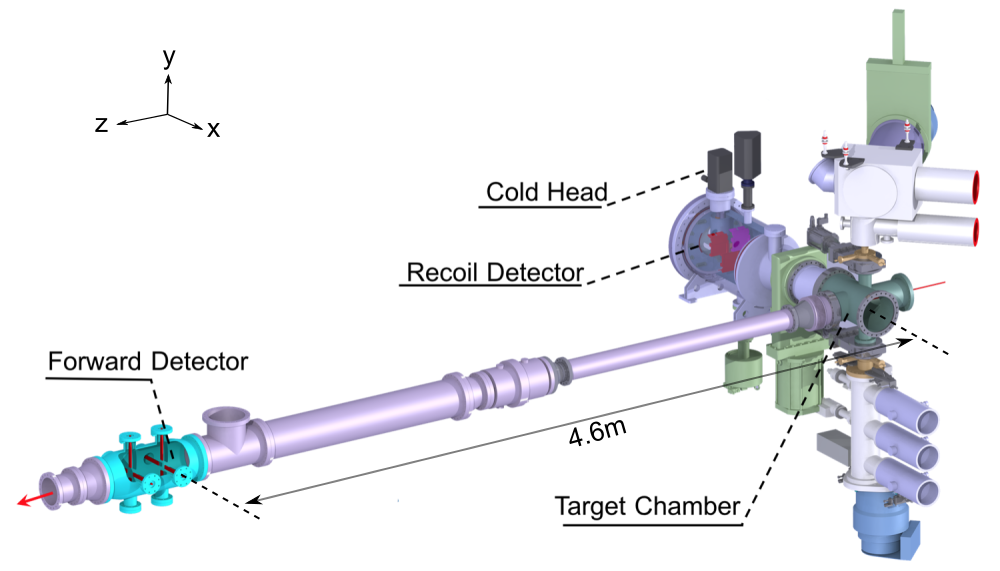
\includegraphics[width=0.8\textwidth]{./koala_setup.png}
	\caption{3D visualization of KOALA setup at COSY}
	\label{fig:setup}
\end{figure*}

The KOALA experiment is a fixed-target experiment aiming to measure the
differential cross-section of $\bar{p}p$ or $pp$ elastic scattering
over the four-momentum transfer range \(0.0008 < |t| < 0.1\) \((GeV/c)^2\).
Due to the identical kinematics of $\bar{p}p$ and $pp$ elastic scattering, the
same setup of KOALA can be used in both measurements.
It is scheduled to measure $\bar{p}p$ elastic
scattering at the future HESR ring of FAIR \cite{FAIR} in the beam momentum range from
1.5 to 15 $GeV/c$.
Before the commission of HESR, KOALA is scheduled to be ran at COSY \cite{COSY}
for measuring $pp$ elastic scattering in the beam momentum range from 1 to 3.7 $GeV$.
Over these beam energy range, KOALA covers the different regions where the Coulomb interaction, the CNI and the nuclear interaction are all significant.
This enables the possibility of the determination of \({\sigma}_{tot}\), \(b\), \(\rho\) as well as
the absolute luminosity by analyzing the characteristic shape of $dN/dt$
spectrum (i.e. relative differential cross section) \cite{bernard1987real,
  jenni2008atlas, recoil_article}.
The absolute differential cross section can be normalized accordingly.

Due to the limitation of beam pipe aperture and the contamination of beam particles,
it is extremely difficult to measure the scattering particle over a wide range of scattering angle in the forward direction.
The recoil measurement technique ,which means precise measurement of  both the recoil angle and the kinematic energy of the recoil proton, 
is used to determine the differential elastic scattering cross section in KOALA.
Identification of the elastic scattering events is based on the match between the recoil angle and the kinematic energy.
A recoil detector prototype based on this idea has already been built
\cite{recoil_article} and the method of recoil measurement technique was verified using proton beams at COSY.
It was also discovered in these tests that the large contamination of low-energy
background events limits the identification of elastic events at very small recoil angles,
which correspond to \(|t| < 0.001\) \((GeV/c)^2\). These backgrounds are mainly
from inelastic scattering processes.

To reach the remaining range \(0.0008 < |t| < 0.001\) \((GeV/c)^2\) in KOALA, a coincidence measurement between the recoil proton and scattering beam particle is proposed to suppress the background contamination.
A time-sensing forward detector with a limited coverage range at small scattering angle is designed and built for this purpose. 
This new setup of KOALA , consisting of the prototype recoil detector, the newly-added forward detector and other upgraded components,  are installed at COSY.
Several tests using proton beams have been carried out to verify the design and the performance.
In the following sections,  the full system of KOALA at COSY is described and the preliminary results from the beam tests are presented.

\section{Experimental setup at COSY}
\label{sec:setup}

KOALA is installed at the previous ANKE segment on the COSY ring.
The setup consists of three arms as shown in Fig. \ref{fig:setup}: the hydrogen
cluster target arm, the recoil arm and the forward arm.
All arms are connected to the target chamber in the center, and they share the same vacuum space as the beam during experiment.

The hydrogen cluster target connects vertically to the target chamber, with the target generator on the top and the target beam dump on the bottom.
The recoil arm is oriented along -X axis of the laboratory frame.
The chamber holding the recoil detector sensors are separated with target
chamber volume with a vacuum gate valve.
This valve is used for staged pumping of the recoil chamber during the
preparation of the experiment and protects the recoil sensors from the residual
gas inside the beam pipe.
The forward chamber connects to the target chamber through one \(\diameter 90
mm\) pipe and one \(\diameter 200 mm\) mm pipe. 

\subsection{Hydrogen cluster target}
\label{sec:target}

A thin and windowless target, which can operate under ultra high vacuum
environment, is critical for the sucess of KOALA.
First, the energy loss of recoil proton before hitting the recoil sensor should
be minimized so that an accurate determination of its kinematic energy is possible.
Second, the thickness of the target (i.e. the profile along the beam direction) determines
the spread of the vertex distribution of beam-target interaction.
Since there is no tracking device in KOALA, the spread will deteriorate the
angular resolution as well as the energy spectrum shape.

The hydrogen cluster target, which is upgraded from the old ANKE target \cite{cluster_target}, is adopted in KOALA.
The collimator is upgraded to a new one and is adjusted to provide a much
smaller width of the cluster beam along the beam axis.
The target thickness is measured to be $\sim2 mm$ in the target chamber center.
The areal density is estimated to be $10^{14} atoms/cm^2$.

\subsection{Recoil detector}
\label{sec:recoil}

The recoil detector needs to totally stop the recoil proton from the
elastic scattering and measure the total energy loss.
For elastic scattering of two particles with the same mass,
the kinematic energy of recoil proton \(T_p\) is proportional to four-momentum
transfer squared by \(|t| = 2m_pT_p\), where \(m_p\) is the proton mass.
For the maximum $|t|=0.1 (GeV/c)^2$, \(T_p \approx 54 MeV\). Thus, a dynamic range of
$0\sim60 MeV$ is required of the recoil detector.

\begin{figure}[htbp]
  \centering
  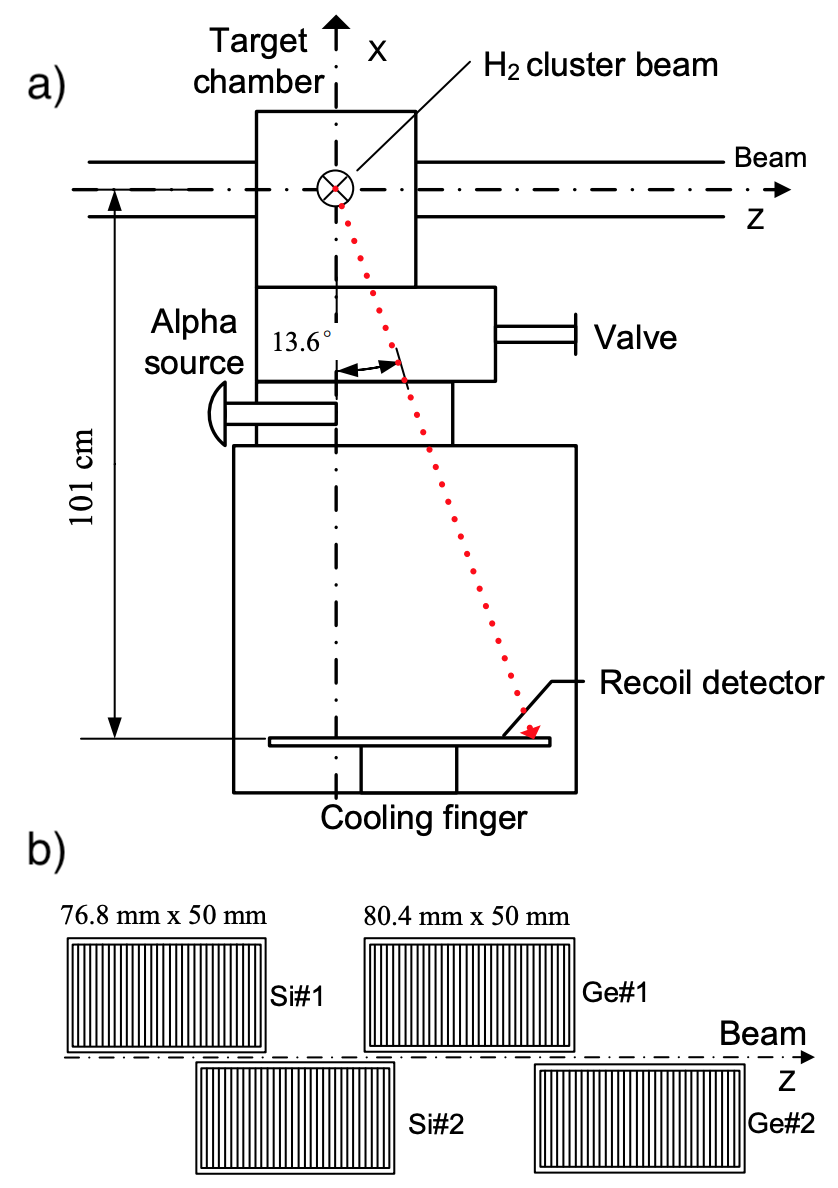
\includegraphics[width=0.4\textwidth]{./recoil_schematic.png}
  \caption{(a) Schematic view of the recoil detector configuration, seen from the
    top; (b) Layout of the four recoil sensors, seen from +X direction}
  \label{fig:recoil_schematic}
\end{figure}

The recoil detector consists of two single-sided silicon strip sensors and two
single-sided germanium strip sensors with a layout shown in Fig. \ref{fig:recoil_schematic}.
The detector plane is installed $90.4 cm$ away from the beam-target center
and covers a range of recoil angle $0\degree < \alpha < 15\degree$.
The sensors are arranged along the beam axis with staggered placement in the Y-axis.
Sensors at different recoil angle have different thickness: $1 mm$ for Si1 and Si2, $5 mm$ for Ge1, $11 mm$ for Ge2.
The silicon sensors have an sensitive area of \(76.8 \times 50 mm^2\), which are
segmented into 64 strips of $1.2 mm$ width.
The germanium sensors have an sensitive area of \(80.4 \times 50 mm^2\), which are segmented into 67 strips of $1.2 mm$ width.
This gives an angular resolution of $\sim0.08\degree$.
Neighboring sensors have an overlapping region which is symmetric against
the beam axis (20 strips for Si1/Si2 overlapping, 9 strips for Si2/Ge1 overlapping, 10 strips for Ge1/Ge2 overlapping).
The overlapping strips are used for the sensor alignment and the correction of beam position asymmetry.

The sensors are readout by a combination of the charge-sensitive preamplifier (MPR16 for the strips, MPR1 for the rear side) 
and the timing filter amplifier (MSCF16), all from Mesytec \cite{mesytec}. 
MSCF16 integrates the shaping amplifier and the leading edge discriminator in the same module.
Both amplitude and timing signal are extracted from MSCF16 for energy and time measurement.
Strips at larger recoil angle are read out by a single channel without sacrificing the angular resolution.
In total, there are 180 readout channels for the recoil detector: 
48 channels on Si1, 64 channels on Si2, 32 channels for Ge1 and Ge2 and 4
channels for the rear sides. 

Soild-state sensors need low and stable operating temperature to optimize energy
resolution.
Temperature of the recoil sensors are monitored by four temperature sensors
attached to the detector holder.
The operating temperature can be actively adjusted by a combination of a cold head and two heating resistors on the cold plate.
A study of the performance of recoil sensors in the laboratory shows that the
optimal working temperature of the recoil detector is $125 K$.
Under this condition, the energy resolutions of the silicon and germanium
sensors are better than $20 keV$ and $30 keV$ (FWHM) respectively.

More technical information and the detailed performance tests of the recoil detector can be found in \cite{recoil_article}.

\subsection{Forward detector}
\label{sec:fwd}

The forward detector aims to to detect the coincident scattering beam proton
from the elastic scattering over the region \(0.0008 < |t| < 0.001\)
\((GeV/c)^2\) and measure its arrival time.

\begin{figure}[htbp]
  \centering
  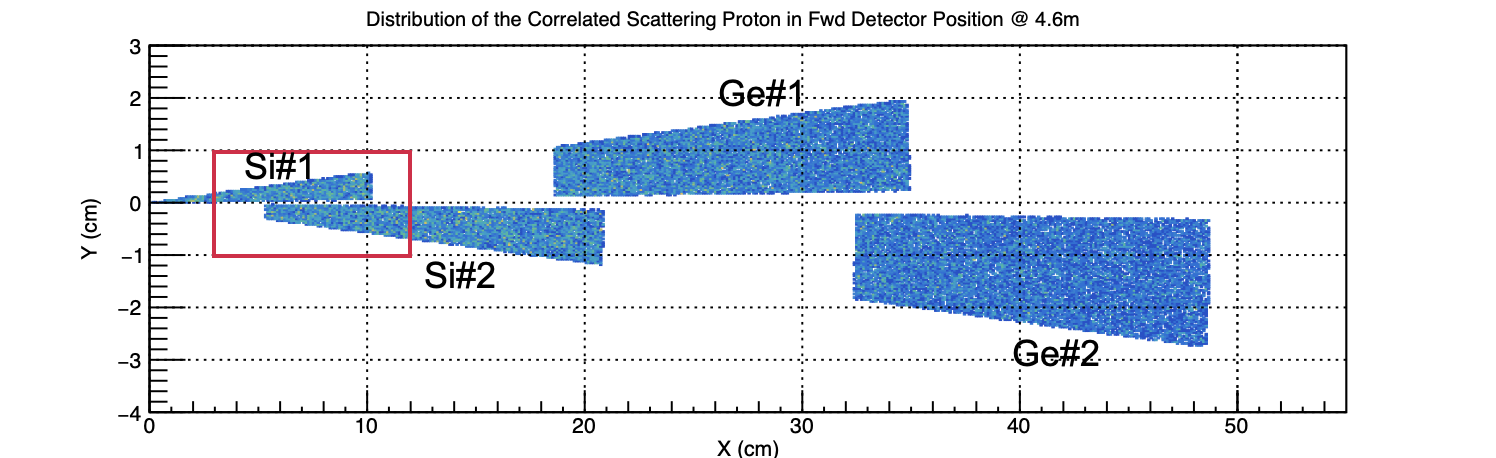
\includegraphics[width=0.45\textwidth]{./fwd_acceptance.png}
  \caption{
    Hit position distribution of the scattering proton on the X-Y plane at $4.6
    m$ from the beam-target center. The results are from the simulation of $2.2
    GeV/c$ $pp$ elasitc scattering with an uniform spherical distribution in the
    center-of-mass reference frame: up) ideal point beam; down) $10mm \times 10mm$ box beam profile.
    % for the elastic scattering events in which
    % the recoil proton hits one of the recoil sensors.
    The four blue blocks are from the events in which the recoil proton hits one of
    the four recoil sensors.
    The red square indicates the size of the forward scintillator, i.e. the covered
    region on the recoil detector by the forward detector.}
  \label{fig:forward_acceptance}
\end{figure}

It consists of 8 detector modules, which are grouped into 2 layers and 4 pairs
as shown inside the forward chamber in Fig. \ref{fig:setup}.
The 4 pairs are installed symmetrically on +X, -X, +Y and -Y axis, with the same
distance of $3 cm$ away from the beam pipe center.
The first layer of each pair are placed $4.6$ downstream the
beam-target center, and the seperation between the two layer is $20 cm$.
Only the pair on -X is used for conincidence detection.
The other 3 pairs are used for beam position tuning during beam preparation and
monitoring during the experiment.
Each module is made of a piece of plastic scintillator (Bicron BC-408
\cite{bc408}) with the dimension \(90 (length) \times 20 (width) \times 6 (thickness)\) mm$^3$.
This gives an acceptance of the scattering angle \(0.37\degree < \theta < 1.49\degree\).
Fig. \ref{fig:forward_acceptance} shows the covered region of the forward detector with an ideal point beam of 2.6 GeV/c.
Most strips on Si1 and a small fraction of strips on Si2 are totally covered.
In real situation, it is expected that fewer
strips will be totally covered with increasing size of beam profile.

\begin{figure}[htbp]
  \centering
  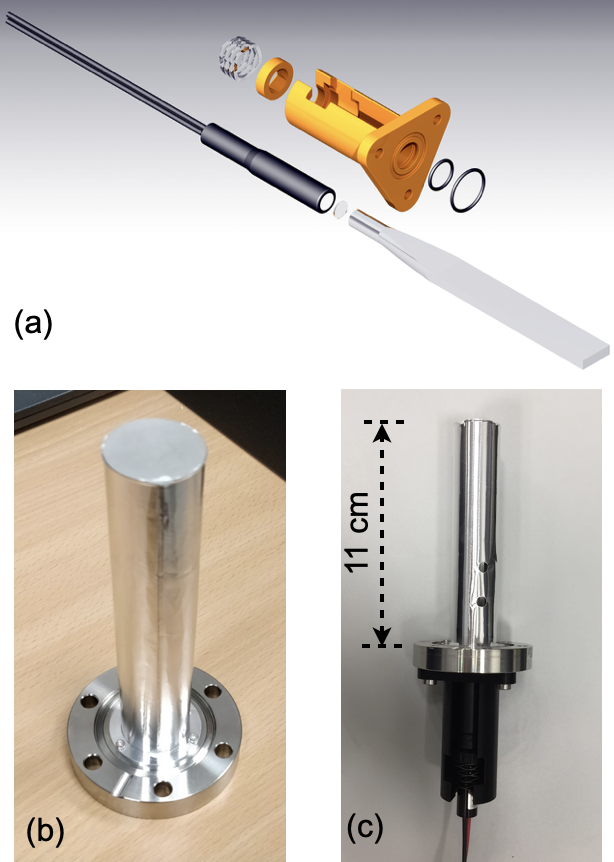
\includegraphics[width=0.32\textwidth]{./forward_module.png}
  \caption{(a) CAD model of the assembly of forward detector module; (b) The aluminum tube is welded on the inside of the flange; (b) One forward detector module after complete assembly}
  \label{fig:forward_module}
\end{figure}

\begin{figure}[htbp]
  \centering
  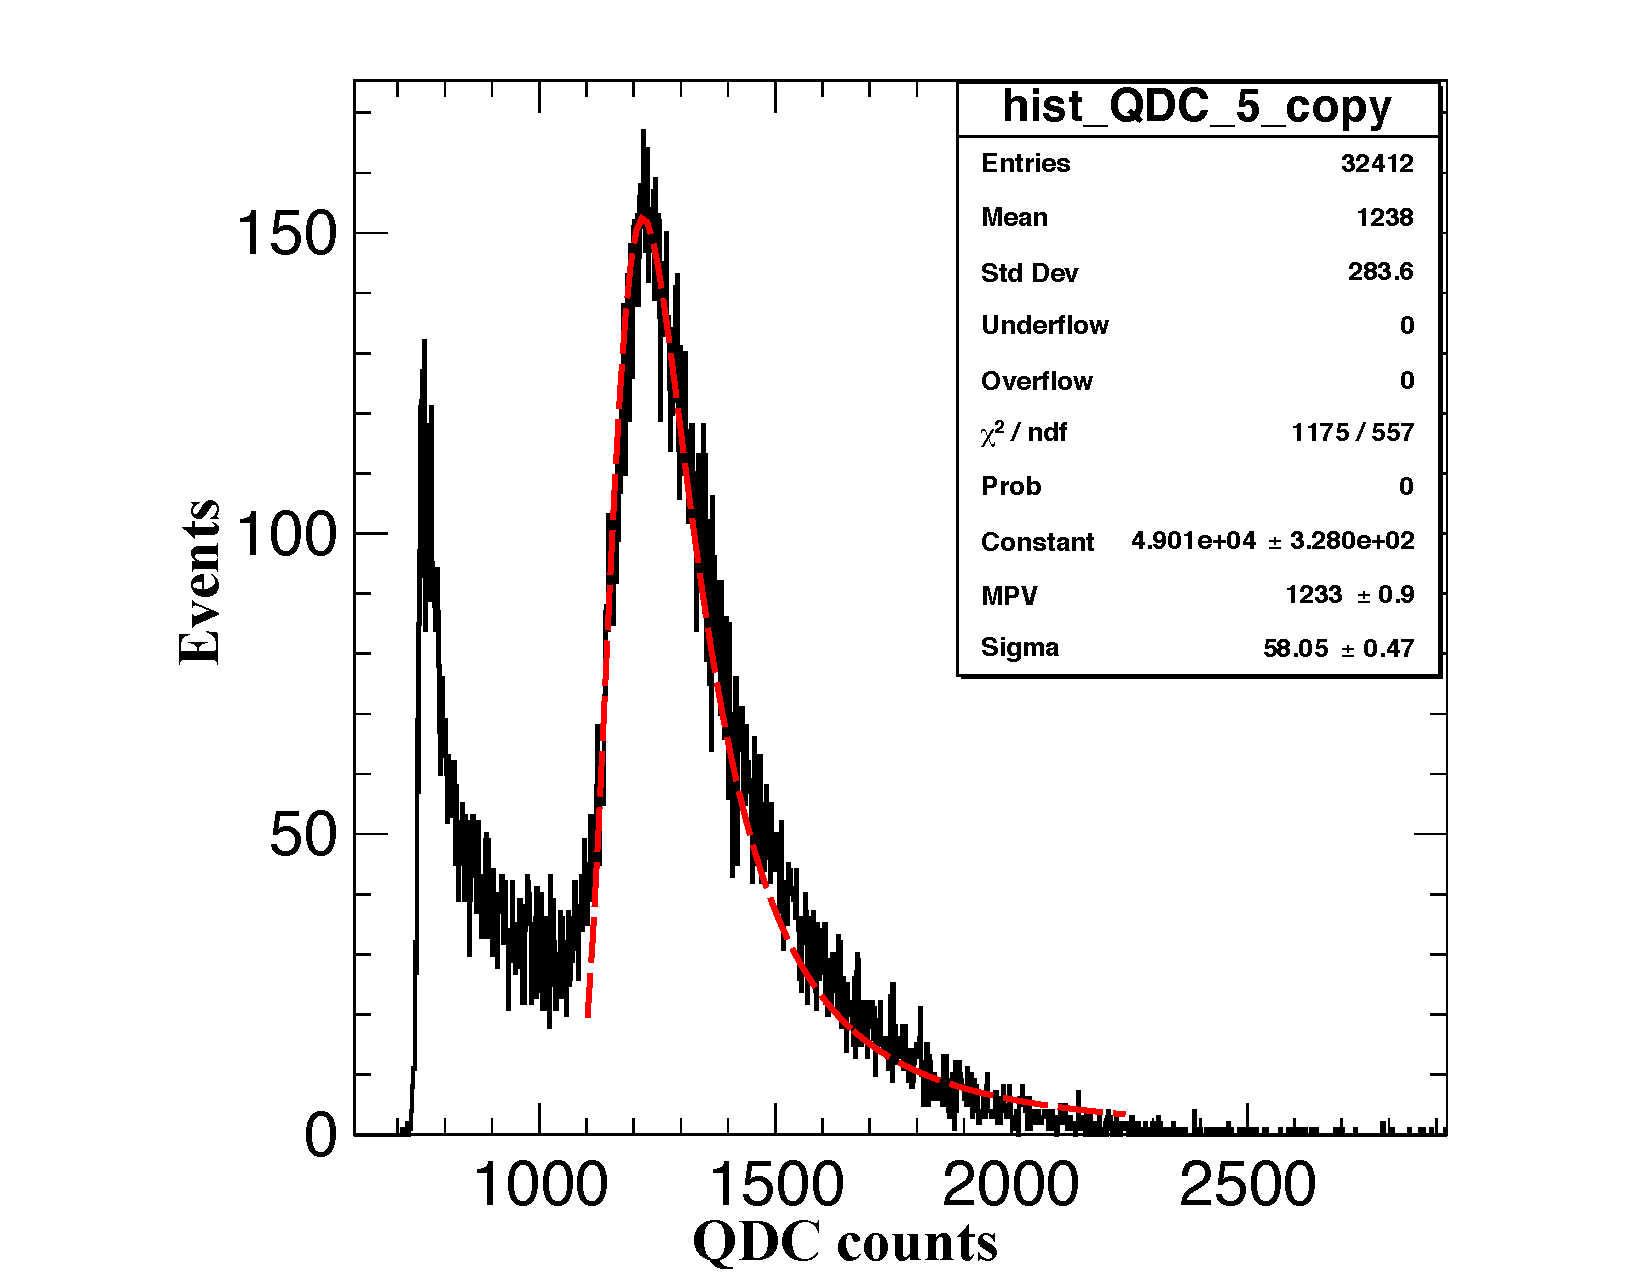
\includegraphics[width=0.4\textwidth]{./forward_mip.pdf}
  \caption{An example of the cosmic ray energy spectrum obtained by a forward detector module prototype}
  \label{fig:forward_mip}
\end{figure}

The scintillator is readout by the combination of a tapered light guide, a piece of silicone pad and a
photomultiplier tube (Hamamastu H6900 \cite{hamamatsu}), as shown in Fig. \ref{fig:forward_module} (a).
Each detector module is integrated with a forward chamber flange for the usage
in the ultra-high vacuum environment.
To protect the vacuum condition inside the beam pipe, the following designs are implemented:
\begin{enumerate}
\item only the light guide and the scintillator are installed inside the forward chamber, the light guide is glued on the open port of the flange as a feedthrough;
\item no wrapping and painting material on the surface of the scintillator, the surface is polished to increase light collection efficiency;
\item a thin aluminum case with thickness of \(100 \mu m\) is used as the light shield of the scintillator, the case is welded on the flange (Fig. \ref{fig:forward_module} (b);
\item two small holes are opened on the side of the aluminum case to speed up vacuum pumping, see Fig. \ref{fig:forward_module} (c).
\end{enumerate}
Other components like the silicone pad, the PMT and the PMT base are installed inside a light-tight case on the other side of the flange as shown in Fig. \ref{fig:forward_module} (c).

Due to the large gain of PMT, no front-end electronics is needed for the readout of the forward detector.
The output signal from H6900 is split into two branches: one fed to a
constant fraction discriminator for time information extraction; the other for charge measurement directly.
Modules are tested using cosmic ray in laboratory before installation.
A typical MIP spectrum obtained by the forward detector module is shown in Fig. \ref{fig:forward_mip}. 
The MIP peak is well separated from the pedestal noise, with signal to noise ratio better than 50.
The timing resolution is measured to be $\sim140 ps$.

\begin{figure*}[htbp]
  \centering
  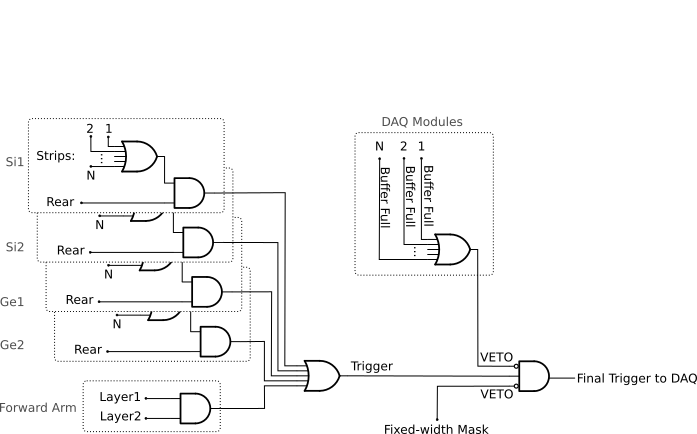
\includegraphics[width=0.75\textwidth]{./trigger_logic.png}
  \caption{Trigger Logic of the KOALA DAQ.}
  \label{fig:trigger_logic}
\end{figure*}

\section{Data acquisition system}
\label{sec:daq}

The data acquisition system of KOALA is a VME-based system with multiple types
of digitization modules provided by Mesytec \cite{mesytec}.
For the recoil detector, the amplitude signal from MSCF16 is digitized by a peak-sensing ADC called MADC-32.
MADC-32 has a 13-bit dynamic range with 6.4 \(\mu s\) conversion time.
For the forward detector, the pulses from PMT are directly fed into a QDC called MQDC-32 for charge measurement.
MQDC-32 has a dynamic range of 500 pC and it uses a 12-bit ADC for digitization with 250 ns conversion time.
The timing information from both the recoil and forward detectors are recorded by a TDC module called MTDC-32 using the conventional Start-Stop method.
MTDC-32 has a minimum resolution of 5 ps.
A multi-channel scalar called SIS3820 \cite{sis} is also integrated to measure
the following key count rates: 1) count rates of the four pairs of the forward detector for beam position monitoring; 2) count rates of the overlapping regions of the recoil detector for asymmetry correction; 3) count rates of the input trigger
for DAQ efficiency correction.

% The acceptance of the forward detector only covers a small part of the recoil detector sensors.
% To record the elastic scattering events from the whole range of the recoil angle
% covered by the recoil detector,
KOALA adopts a self-triggering scheme for the trigger logic design.
Each sensor of the recoil detector and each arm of the forward detector works independently and generates their own trigger. 
The final trigger to the DAQ is a common OR of all sub-detectors, as shown in Fig. \ref{fig:trigger_logic}.
The trigger from the recoil detector sensor is generated by a coincidence between the front-side strips and the rear-side plane, 
and the trigger from the forward detector arm is generated by a coincidence between the two modules in the same pair.
% In this way, the rate of the false hits generated by electronic noise can be minimized.
Both elastic and inelastic scattering events are recorded in this trigger design, and the coincidence between the recoil sensor and the forward detector is carried out in offline analysis.

Fast readout of the recorded event is crucial for a self-triggered DAQ system.
The asynchronous readout mechanism combined with VME CBLT block read mode is adopted to increase the data throughput in KOALA.
The digitization modules used in KOALA all have an event buffer with a size $> 32 kB$.
Digitized events are stored in this buffer before readout, so that the module is immediately available to digitize the next event.
Events will not be readout until the buffer is nearly full.
Since the cross section is higher at smaller recoil angle, the module for these channels always saturates faster than others.
Modules with a saturated event buffer may miss new coming events while others
not, and thus bringing a systematic bias.
To overcome this issue, the buffer-full signal from each module is added to the trigger logic as VETO as shown in Fig. \ref{fig:trigger_logic}.

The issue about event synchronization arises naturally when using asynchronous
readout mode.
% The digitization modules used in KOALA have different dead time, especially between MADC-32 and MTDC-32.
% An event recorded by a fast module may be missed by a slow module. This creates un-synchronous event structure, which makes the sequential event data assembling impossible. 
Timestamp-based synchronization is used to solve this problem.
The modules in the system have a 30-bit counter for recording the timestamp from
the clock signal distributed by a central source.
The source could be either the VME built-in clock ($16 MHz$) or an external clock
($< 75 MHz$).
Currently, the built-in clock of VME backplane bus is used. 
Based on this timestamp, event synchronization is achieved offline.
The other option is adding a fixed-width mask gate into the trigger logic as VETO, as show in Fig. \ref{fig:trigger_logic}.
The width of the mask gate should be larger than the maximum dead time of all modules.
In this way, the events are effectively synchronized sequentially. 
However, this method may reduce DAQ efficiency significantly in a high hit-rate environment.

\begin{figure}[htbp]
\centering
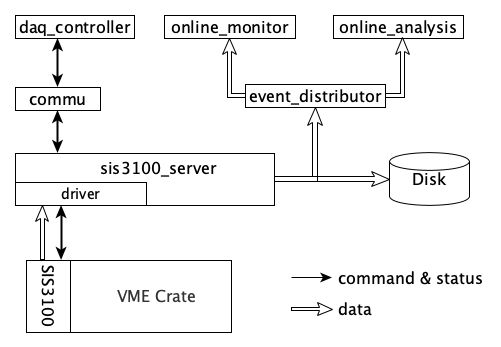
\includegraphics[width=0.45\textwidth]{./koalaems_deployment.png}
\caption{Design and deployment of KoalaEms.}
\label{fig:koalaems}
\end{figure}

A dedicated DAQ software called KoalaEms is also developed for KOALA.
KoalaEms is a fork of the EMS software \cite{ems}, which is a highly flexible DAQ software framework developed for various experiments at COSY.
Support for the VME controller (SIS3100 \cite{sis}) is integrated and a new component of online monitoring based on ROOT is added.
The architecture of KoalaEms is shown in Fig. \ref{fig:koalaems}.
The interface to the DAQ is implemented as \emph{sis3100\_server}, the host of which
connects to SIS3100 by an optical link.
The control and status information from/to the GUI \emph{daq\_controller} is mediated by a component called \emph{commu}.
The data flow from VME crate is split into two branches: 1) \emph{data\_out\_disk}: save the raw data onto disk; 2) \emph{data\_out\_stream}: stream out to \emph{event\_distributor}.
\emph{event\_distributor} will forward the data stream to various consumption hosts for usages like online monitoring and online analysis.
Both \emph{commu} and \emph{event\_distributor} support socket connection and the \emph{event\_distributor} also supports multiplexing streaming.
All the square blocks in Fig. \ref{fig:koalaems} can be hosted in different PC and new consumption host to the data stream can be integrated whenever needed.


\section{Software framework}
\label{sec:software}

A dedicated software framework called KoalaSoft is developped for the simulation, calibration, reconstruction and analysis jobs of the KOALA experiment.
It is built upon the FairRoot \cite{fairroot} framework, which implements a simulation environment based on VMC \cite{vmc} library and an analysis environment based on ROOT's task concept.
The components stack of KoalaSoft is shown in Fig. \ref{fig:koalasoft}.

\begin{figure}[htbp]
  \centering
  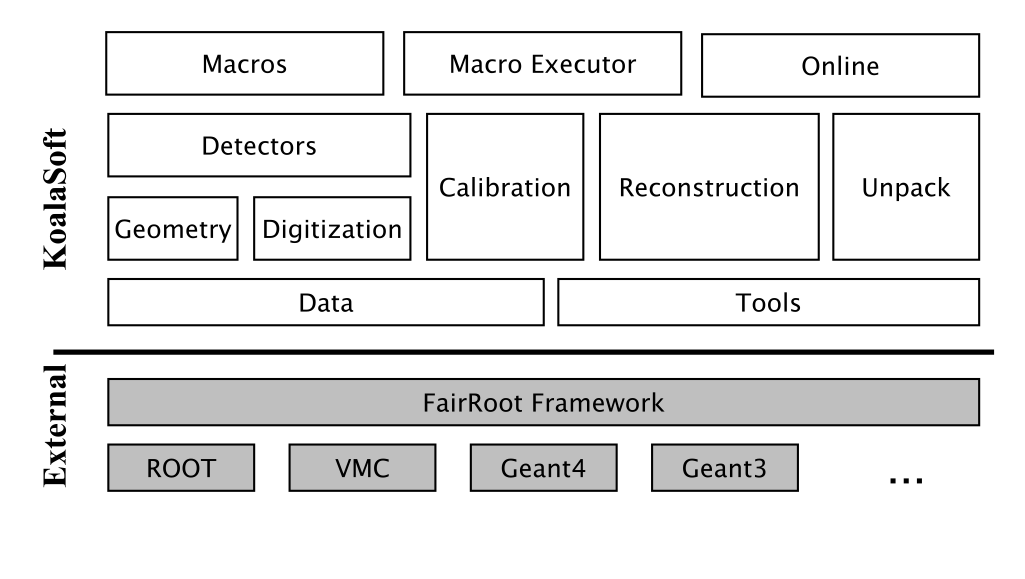
\includegraphics[width=0.48\textwidth]{./koalasoft_components.png}
  \caption{Components of KoalaSoft}
  \label{fig:koalasoft}
\end{figure}

Both Geant3 and Geant4 can be selected as the simulation engine without changing other components in KoalaSoft.
Geometry models of the recoil detector and the forward detector are implemented using ROOT's TGeo library.
Jobs like digitization, calibration and reconstruction are divided into multiple smaller steps, each of which is represented by a single task.
Tasks chained together later in a ROOT macro to compose a full job. 
ROOT macros are the interface for the end user using KoalaSoft.
Macros for common jobs are pre-configured and distributed along with KoalaSoft.
Users can also compose their own specific jobs for analysis.
Additionally, a binary macro executor is provided to run jobs directly from command line. This may be useful in batch processing.

In KoalaSoft, the same chain of tasks can be used for the analysis of both the simulation data and the raw data from DAQ.
This is accomplished by the \emph{Unpack} component, which can decode and transform the raw binary data into the same format as the output from simulation jobs.
Algorithms developped, tested and verified using simulation data be applied to experimental data seamlessly.
This saves a lot of efforts in the development and maintainence of algorithms.
Both the offline disk data and the online streaming data are correctly handled by \emph{Unpack} and an online monitoring program is developped based on it.

\section{Reconstruction}
\label{sec:reconstruction}

\subsection{Energy calibration}
\label{sec:calibration}

\begin{figure*}[htbp]
\centering
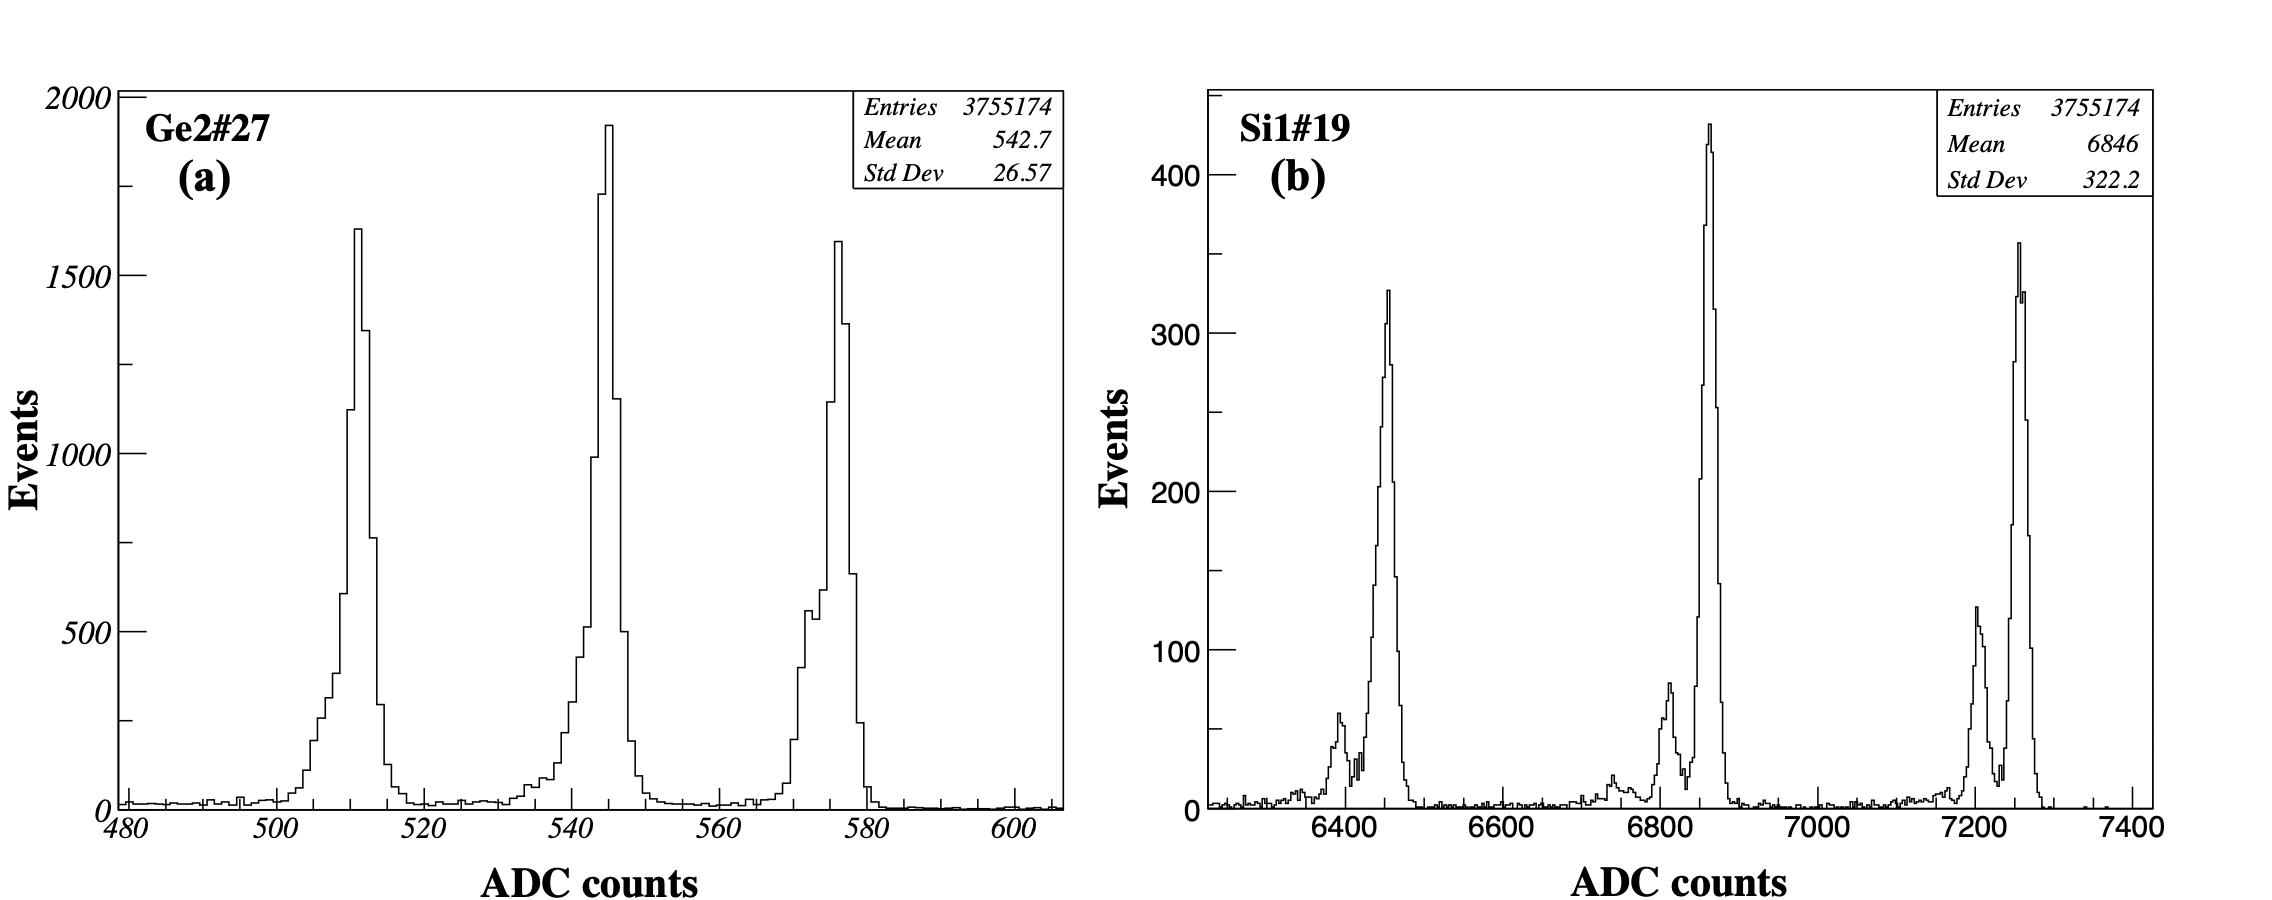
\includegraphics[width=0.8\textwidth]{./alpha_response.png}
\caption{Example energy spectrums of \(\alpha\) sources of two channels at different positions: (a) large recoil angle $13.9\degree$; (b) small recoil angle $0.93\degree$}
\label{fig:alpha_spectrum}
\end{figure*}

% Precise measurement of energy deposit in the recoil detector is critical for the
% identification of elastic scattering events as well as the calculation of the recoil angle.
\(\alpha\) sources \(^{239}Pu\), \(^{244}Cm\), \(^{241}Am\), with decay energies of 5156.59 keV, 5804.83 keV, 5485.56 keV \cite{nuclear_data} respectively, are used for the energy calibration.
Decays with much smaller branch ratios also exist in these sources. They may also be used in the energy calibration if they are well separated from the main peaks.
$\alpha$ sources are installed inside the recoil chamber and fixed on a linear motion feedthrough rod.
During experiment, the rod is lifted and the sources are blocked by the chamber wall;
when calibration is needed, the rod is pushed to the chamber center and the sources face the recoil sensors directly.
Thus, the recoil detector can be calibrated regularly after commissioning of KOALA.

Two aspects need special consideration in the calibration.
First, the recoil sensors have a protective layer on the surface. 
\(\alpha\) particles will lose some energy in this layer before entering the
fiducial volume of the sensor.
The thickness of the protection layer has been measured in the laboratory using \(\gamma\) rays \cite{recoil_article}.
The energy loss in the protection layer is calculated and shown in Tab. \ref{tab:dead_layer} for each $\alpha$ energy when the incidence angle is $90\degree$.
The effective energy deposit in the fiducial volume is further corrected based
on the recoil angle of each strip.

\begin{table}[htbp]
\label{tab:dead_layer}
\caption{Energy loss (keV) of $\alpha$ in the protection layer when incidence angle is $90\degree$}
\centering
\begin{tabular}{cccccc}
\hline
\(E_{\alpha} (keV)\) & \(\Delta E_{Si1}\) & \(\Delta E_{Si2}\) & \(\Delta E_{Ge1}\) & \(\Delta E_{Ge2}\) \\
\hline
5156.59 & 11.51 & 11.51 & 110.00 & 111.00 \\
5485.56 & 11.01 & 11.01 & 105.00 & 106.00 \\
5804.83 & 10.52 & 10.52 & 99.00  & 100.00 \\
\hline
\end{tabular}
\end{table}

Secondly, the gain setting of each readout channel is optimized for the recoil
energy range covered by the strip.
The gain difference can vary up to a factor of ~10.
Thus, the resolution is worse at large recoil angle than at small angle, as shown in Fig. \ref{fig:alpha_spectrum}.
The minor decay modes can't be recognized in Fig. \ref{fig:alpha_spectrum} (a), while they are clearly seen in Fig. \ref{fig:alpha_spectrum} (b).
Since only three energy points can be used, Lower resolution brings larger systematic error in the calibration.

\begin{figure}[htbp]
\centering
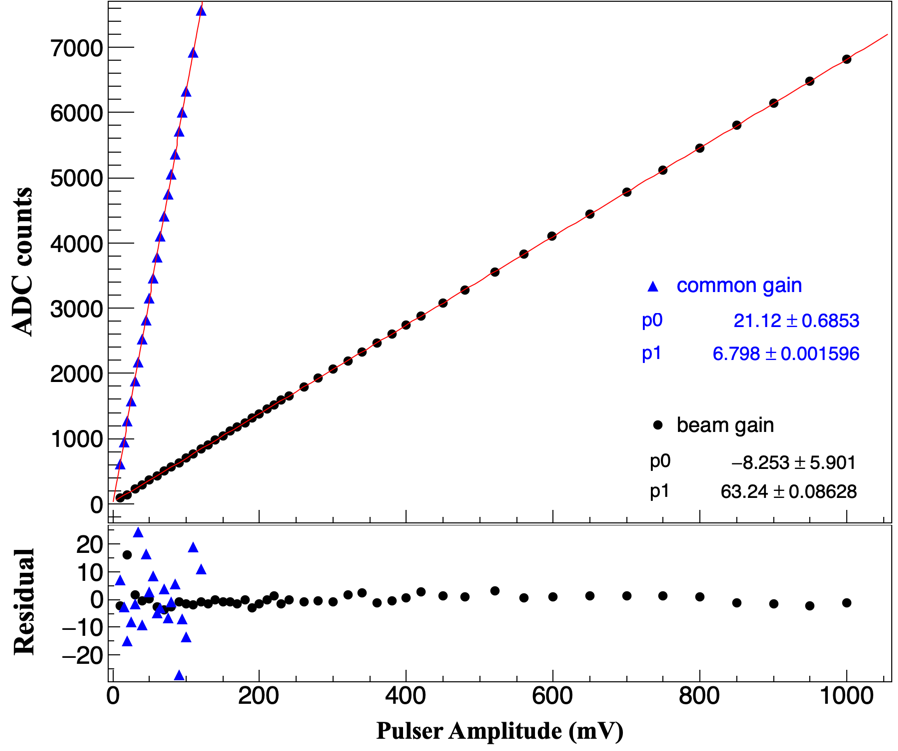
\includegraphics[width=0.42\textwidth]{./linearity.png}
\caption{Electronic linearity of a typical recoil detector channel}
\label{fig:electronic_linearity}
\end{figure}

To minimize this error, a common gain, which is optimized for the separation of the \(\alpha\) energy peaks, is set for all channels.
The calibration is carried out as follows:
\begin{enumerate}
\item the energy spectrum of the \(\alpha\) sources is recorded under the common gain setting and the energy peaks are searched;
\item the gain difference between the common gain and the beam gain setting used
  in experiment is measured by scanning a precision analog pulser over a large range of amplitudes;
\item the energy responses at beam gain setting are then deduced by applying the gain
  difference to the common gain responses, and the result is fitted using a linear function.
\end{enumerate}
The fitting parameters of the last step are the parameters used to convert ADC
values into energy in the reconstruction.
The electronics of recoil detector has a very good linearity in both gain
settings, as shown in Fig. \ref{fig:electronic_linearity}. 
Thus, this indirect method is reliable and the systematic error of the
calibration is reduced.

\subsection{Time walk correction}
\label{sec:timewalk}

Time walk effect of the leading edge discriminator used in the recoil detector needs to be corrected to
optimize the timing resoultion.
Calibration of the time-walk effect is carried out using a  precision analog pulser. 
Output of the pulser is split into two branches: one is fed into a constant fraction discriminator to generate the reference time;
the other is connected to the detector channel under calibration for measurment. 
By scanning the pulser over a wide range of amplitudes, the time-walk effect is
revealed.
An example is shown in Fig. \ref{fig:timewalk}, where the result is fitted with \(y=p_0 x^{-1} + p_1\). 
The time walk is corrected by substracting \(\Delta t = p_0/ADC\) from the
measured timing value.

\begin{figure}[htbp]
  \centering
  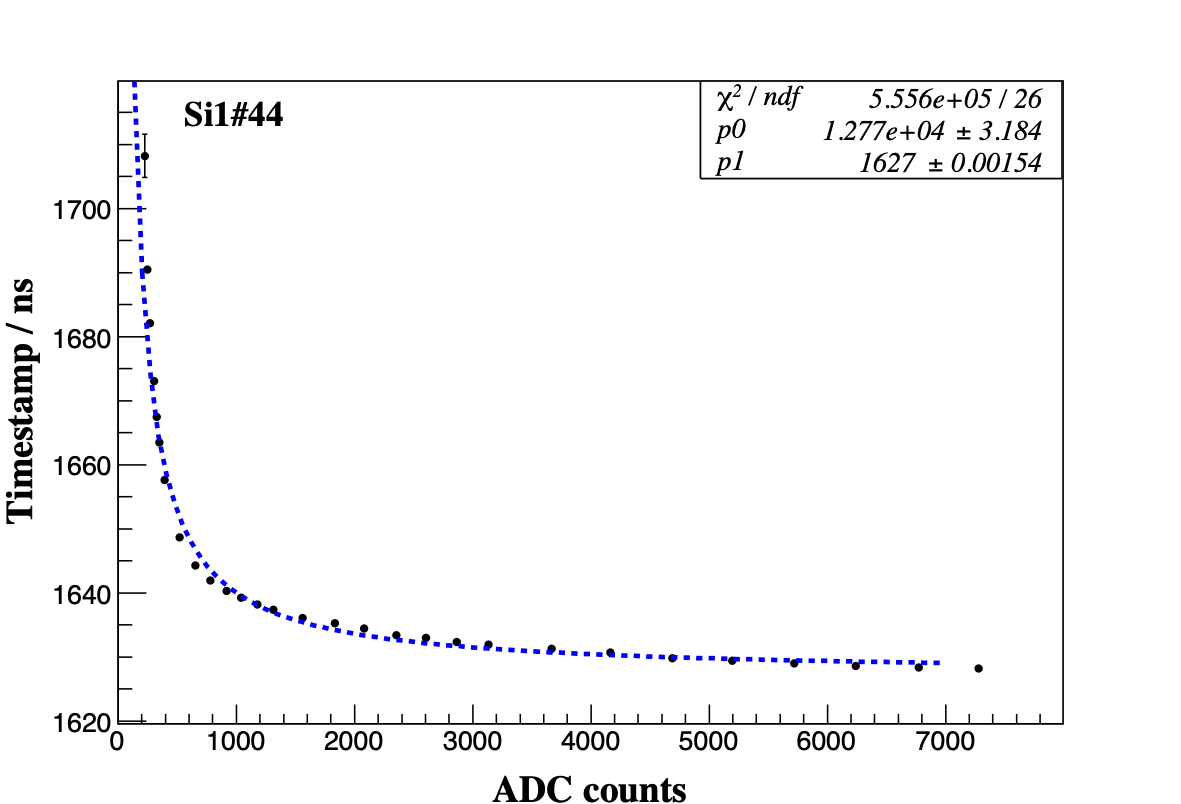
\includegraphics[width=0.45\textwidth]{./timewalk.png}
  \caption{Typical result from the time-walk calilbration.}
  \label{fig:timewalk}
\end{figure}

Moreover, the difference of the fitting paramter \(p_1\) indicates the delay time
difference between different channels, which is caused by the signal routing length variation.
These offsets are also applied in the reconstruction to align the timing from different channels.

\subsection{Clustering}
\label{clustering}

Clustering is necessary to reconstruct the correct energy deposit in the
recoil detector for the following reasons: 1) charge sharing is an intrinsic characteristic of solid-state strip detector, especially
for the tracks hitting the edge in between the adjacent strips; 2) the tracks
from beam-target interaction may penetrate through several strips before
stopping, especially for the sensors at large recoil angle (simulation shows
that ~50\% of the tracks hitting Ge2 have hit multiplicity larger than 1).

The clustering algorithm is designed to minimize the noise contribution while
at the same time keeping the low-energy background characteristic as much as possible.
It is also important not to bring a selection bias between low energy and high energy elastic events.
The steps of clustering in KOALA is as follows:
\begin{enumerate}
\item Delete noise hits. Hits induced by the electronic noise is deleted. A low
  threshold ($2\sigma_{noise}$) is used in this step.
\item Collect remaining hits into clusters based on the adjacency principle.
\item Delete noise clusters. The noise level of cluster is evaluated as
  $\sigma_{cluster} = \sum_i^n{\sigma_{noise}^i}$, where $\sigma_{noise}^i$ is
  the noise level of each strip in the cluster. Clusters which have summed
  energy lower than $5\sigma_{cluster}$ are considered to be noise-induced and deleted.
\item Delete clusters without seed hit. Valid cluster needs to have at lease one seed hit, the
  amplitude of which exceeds the equivalent energy of the trigger threshold of
  the corresponding strip.
\end{enumerate}

\section{Test beam results}
\label{sec:result}

Beam tests were carried out using proton beam with momentum 2.2, 2.4, 2.6 and
3.0 GeV/c in August and October, 2019.
\begin{figure}[h]
  \centering
  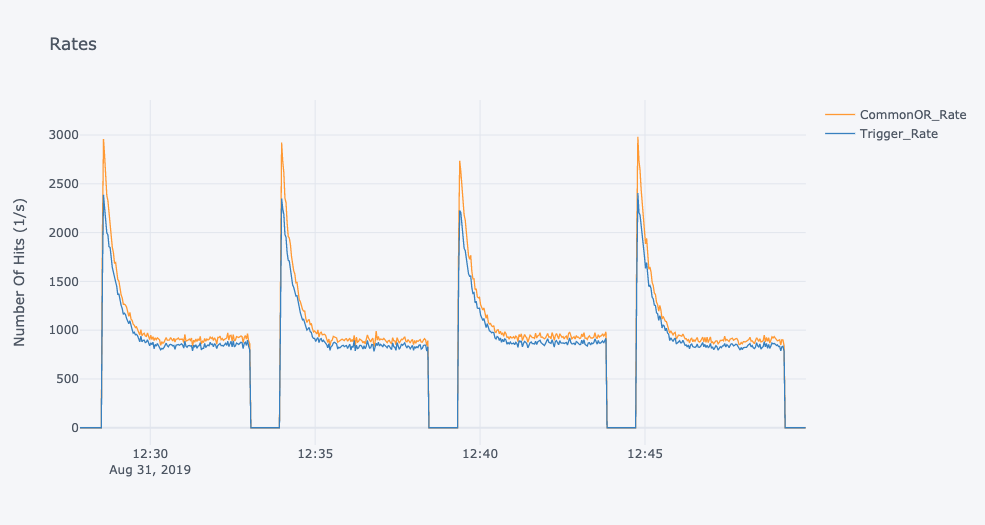
\includegraphics[width=0.45\textwidth]{./daq_efficiency.png}
  \caption{Beam cycle and DAQ efficiency.}
  \label{fig:beam}
\end{figure}
The beam intensity is about $10^{10}$ s$^{-1}$, with an cycle structure of
$\sim40 s$ injection time and $\sim300 s$ storage time, as shown in Fig. \ref{fig:beam}.
% During injection cycle, the beam has large emittance and not stable.
Only the storage cycle is used for the experiment, which is achieved by two
gates synchronized with the beam cycle.
One gate is used to protect the PMTs of the forward detector, which ramps down the high voltage supply $5s$ before the end of the
storage cycle and ramps up the high voltage supply $5s$ after the start of the storage cycle.
The other gate has a narrower width and is used to control the data
acquisition system so that data are not recorded during injection.
Stochastic beam cooling is also applied to minimize the size of beam profile.
It reaches the equibilium state after the beginning 1/3 of the experiment cycle.
Fig. \ref{fig:beam} also shows the DAQ efficiency in variation with the input trigger rate.
A maximum of 93\% is reached ,which amounts to 850 events/s.
% The efficiency is mainly limited by a wide mask gate in the trigger logic.

The analysis of the test beam data are same for all beam energies.
In the following, the results from 2.2 $GeV/c$ are shown as example.
Typical energy spectrums of the recoil detector are summarized in Fig.
\ref{fig:e_map}.
\begin{figure}[htb!]
  \centering
  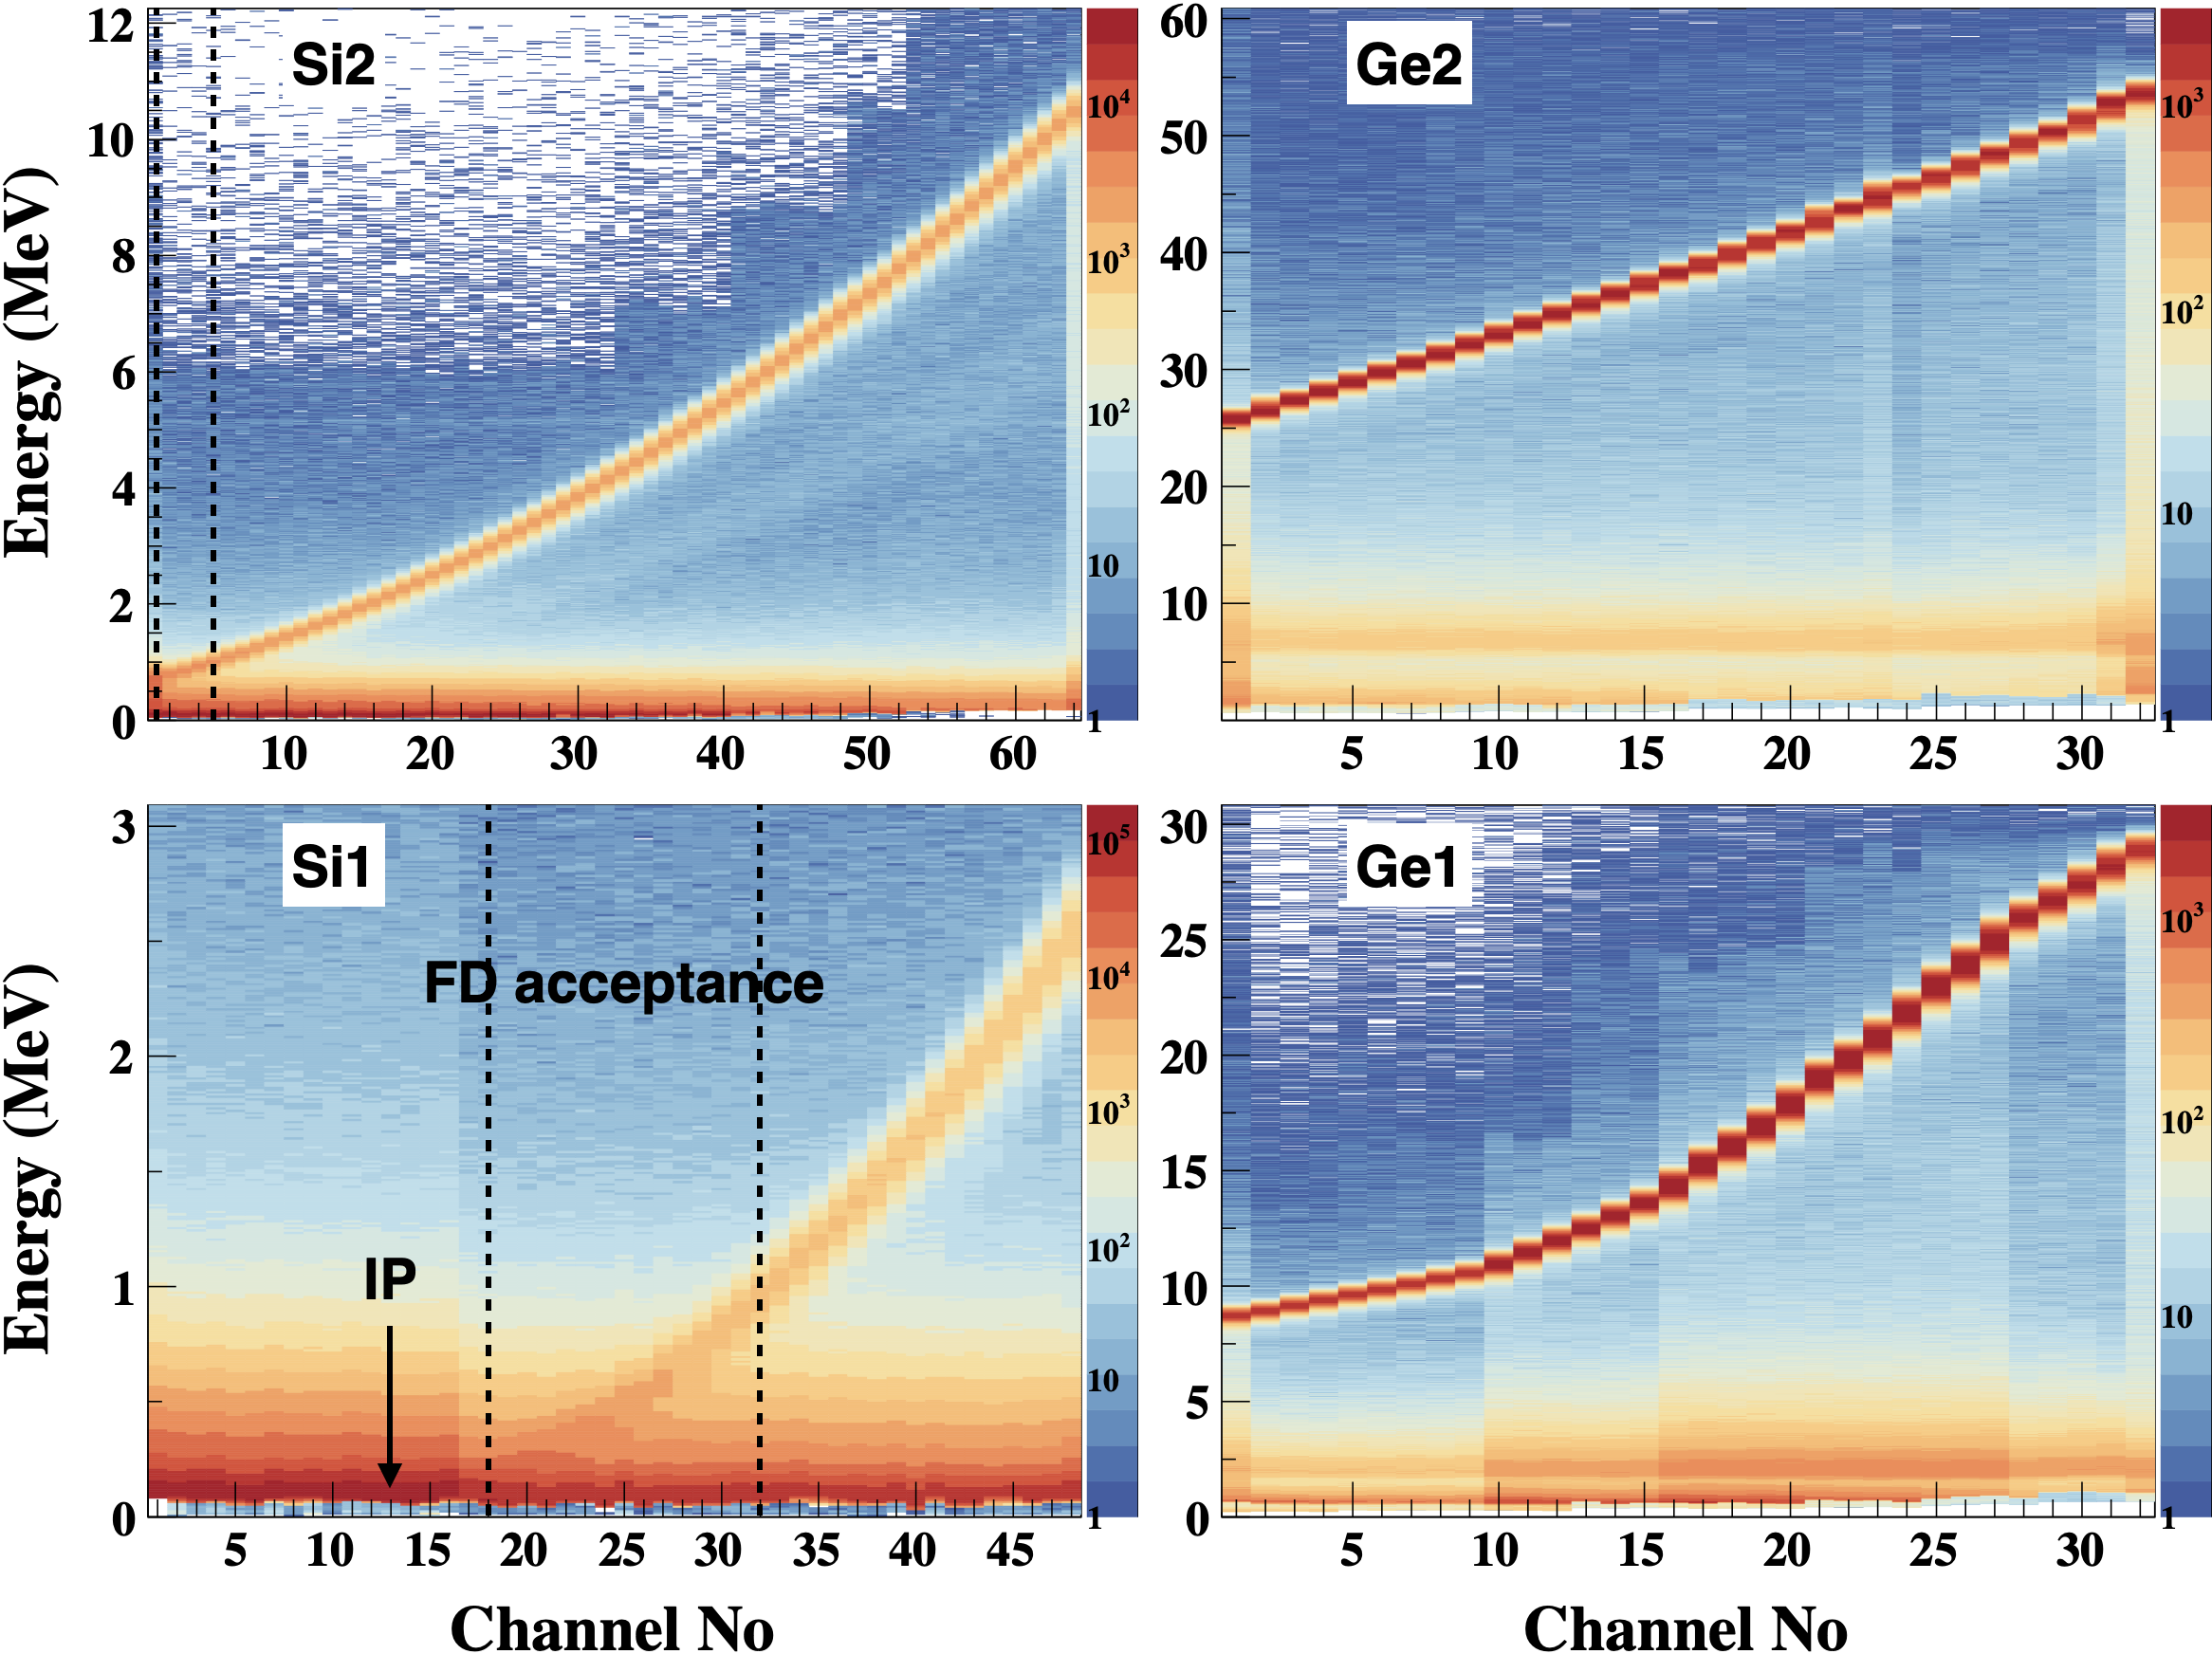
\includegraphics[width=0.5\textwidth]{./e_map.png}
  \caption{Energy spectrums (after clustering) of all channels of the 4 recoil
    sensors at 2.2 GeV/c.  IP indicates the channel which is in alignment with
    the beam-target center. Channel 22 and 23 of Ge2 are channels with
    malfunctional electronics.
    % The group of channels of Si1 and Si2 which are fully covered by the forward detector are indicated.
  }
  \label{fig:e_map}
\end{figure}
The pattern of the recoil energy variation of elastic scattering events with respect to the channel position is observed.
For most channels of the recoil detector, the elastic peaks are clearly
separated from the low-energy background
and can be extracted with an appropriate background model as shown in Fig. \ref{fig:e_fit}.
\begin{figure}[h!]
  \centering
  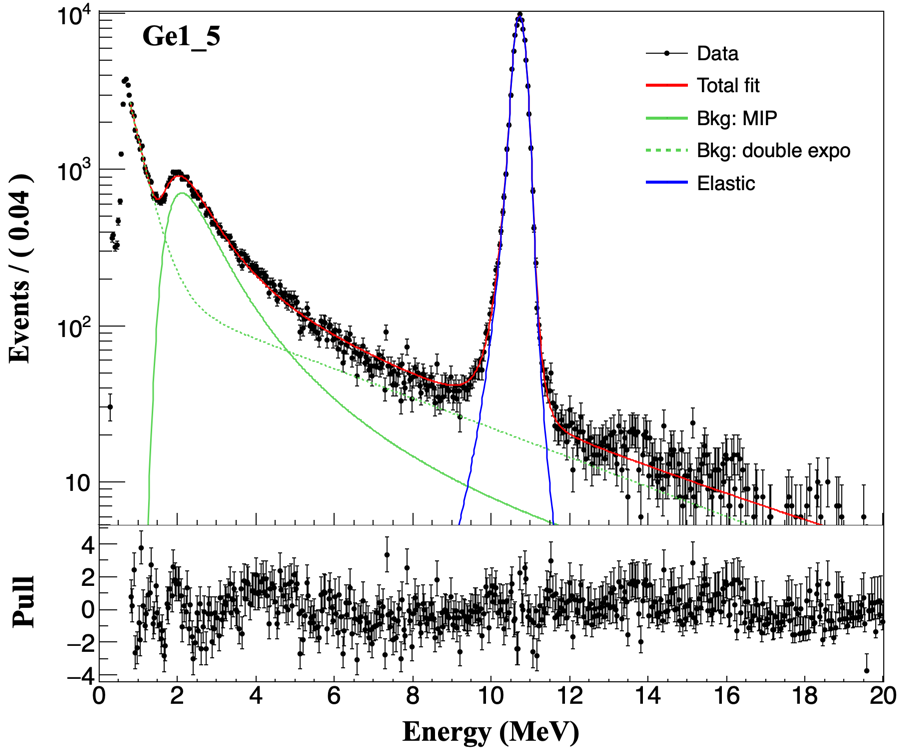
\includegraphics[width=0.42\textwidth]{./e_fit.png}
  \caption{An example of the fit result with background model: MIP + double
    exponential decay.}
  \label{fig:e_fit}
\end{figure}
Most of the remaining channels, in which the elastic peak can't be easily identified from the
background, are fully covered by the forward detector as indicated in Fig. \ref{fig:e_map}.
For these channels, the coincidence between the recoil proton and the forward
scattering can be used.


The time-of-flight (TOF) of the recoil proton and its kinematic energy (E)
follows a definite relation $TOF = l\sqrt{m_p/2E}$, where $l$ is the distance of
the recoil detector to the interaction point, $m_p$ is the proton mass.
Due to the small flight-time variation of the forward scattering proton, TOF of the recoil proton can be approximated by the difference
between the timestamp of the recoil detector and the forward detector.
A typical TOF-E spectrum obtained from the tests is shown in Fig. \ref{fig:tof-e}, in which the elastic
events are recognized as the peak band in the center.
\begin{figure}[h!]
  \centering
  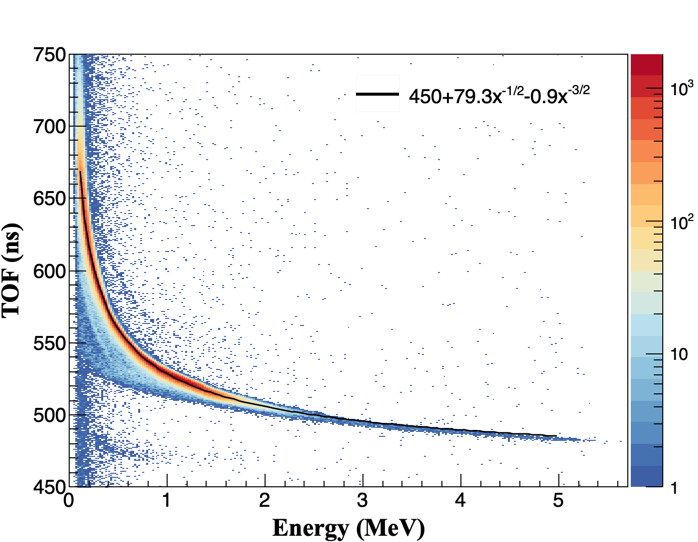
\includegraphics[width=0.45\textwidth]{./tof_e_cut.png}
  \caption{
    TOF-E spectrum of the recoil proton at 2.2 GeV/c. The data is from all
    strips which are either fully or partly covered by the forward detector.}
  \label{fig:tof-e}
\end{figure}
The events lying outside of the peak band are from inelastic processes and
they overlap with the elastic events at very small recoil energy (i.e. small recoil angle) when projected to the energy spectrum.
The elastic band is fitted with the model $y = p_{0} + p_{1}x^{-1/2} + p_{2}x^{-3/2}$,
which describe the data very well above $0.1 MeV$.
% The third term in the fit model is brougt in for correcting the approximation.

% To select the elastic events, the fit result of the TOF-E is moved up and down to form a selection region as shown in the pink curves in Fig. \ref{fig:tof-e}.
Using the fitted TOF-E relation as reference, a selection window is composed
based on the standard deviation of TOF spectrum profile for each channel.
The elastic peak is filtered out from a large background after applying the selection window, as shown in Fig. \ref{fig:cut}.
More accurate fit of the elastic spectrum can be carried out with the new spectrum.
Applying this method to all channels covered by the forward detector, the lowest
measurable energy can be deduced.
Fig. \ref{fig:measured_vs_calculated} shows the comparison between the measured
energy of the elastic peak and the expected energy of the recoil proton from elastic scattering at 2.2 GeV/c.
A limit is observed around \(200 keV\), which corresponds to $|t| \approx  0.0004  ((GeV/c)^2$.
Same analysis on other three beam momentums shows that the minimum measurable
recoil energies are all below $300 keV$, which is well beblow the desired $|t|_{min}$.

\begin{figure}[h!]
  \centering
  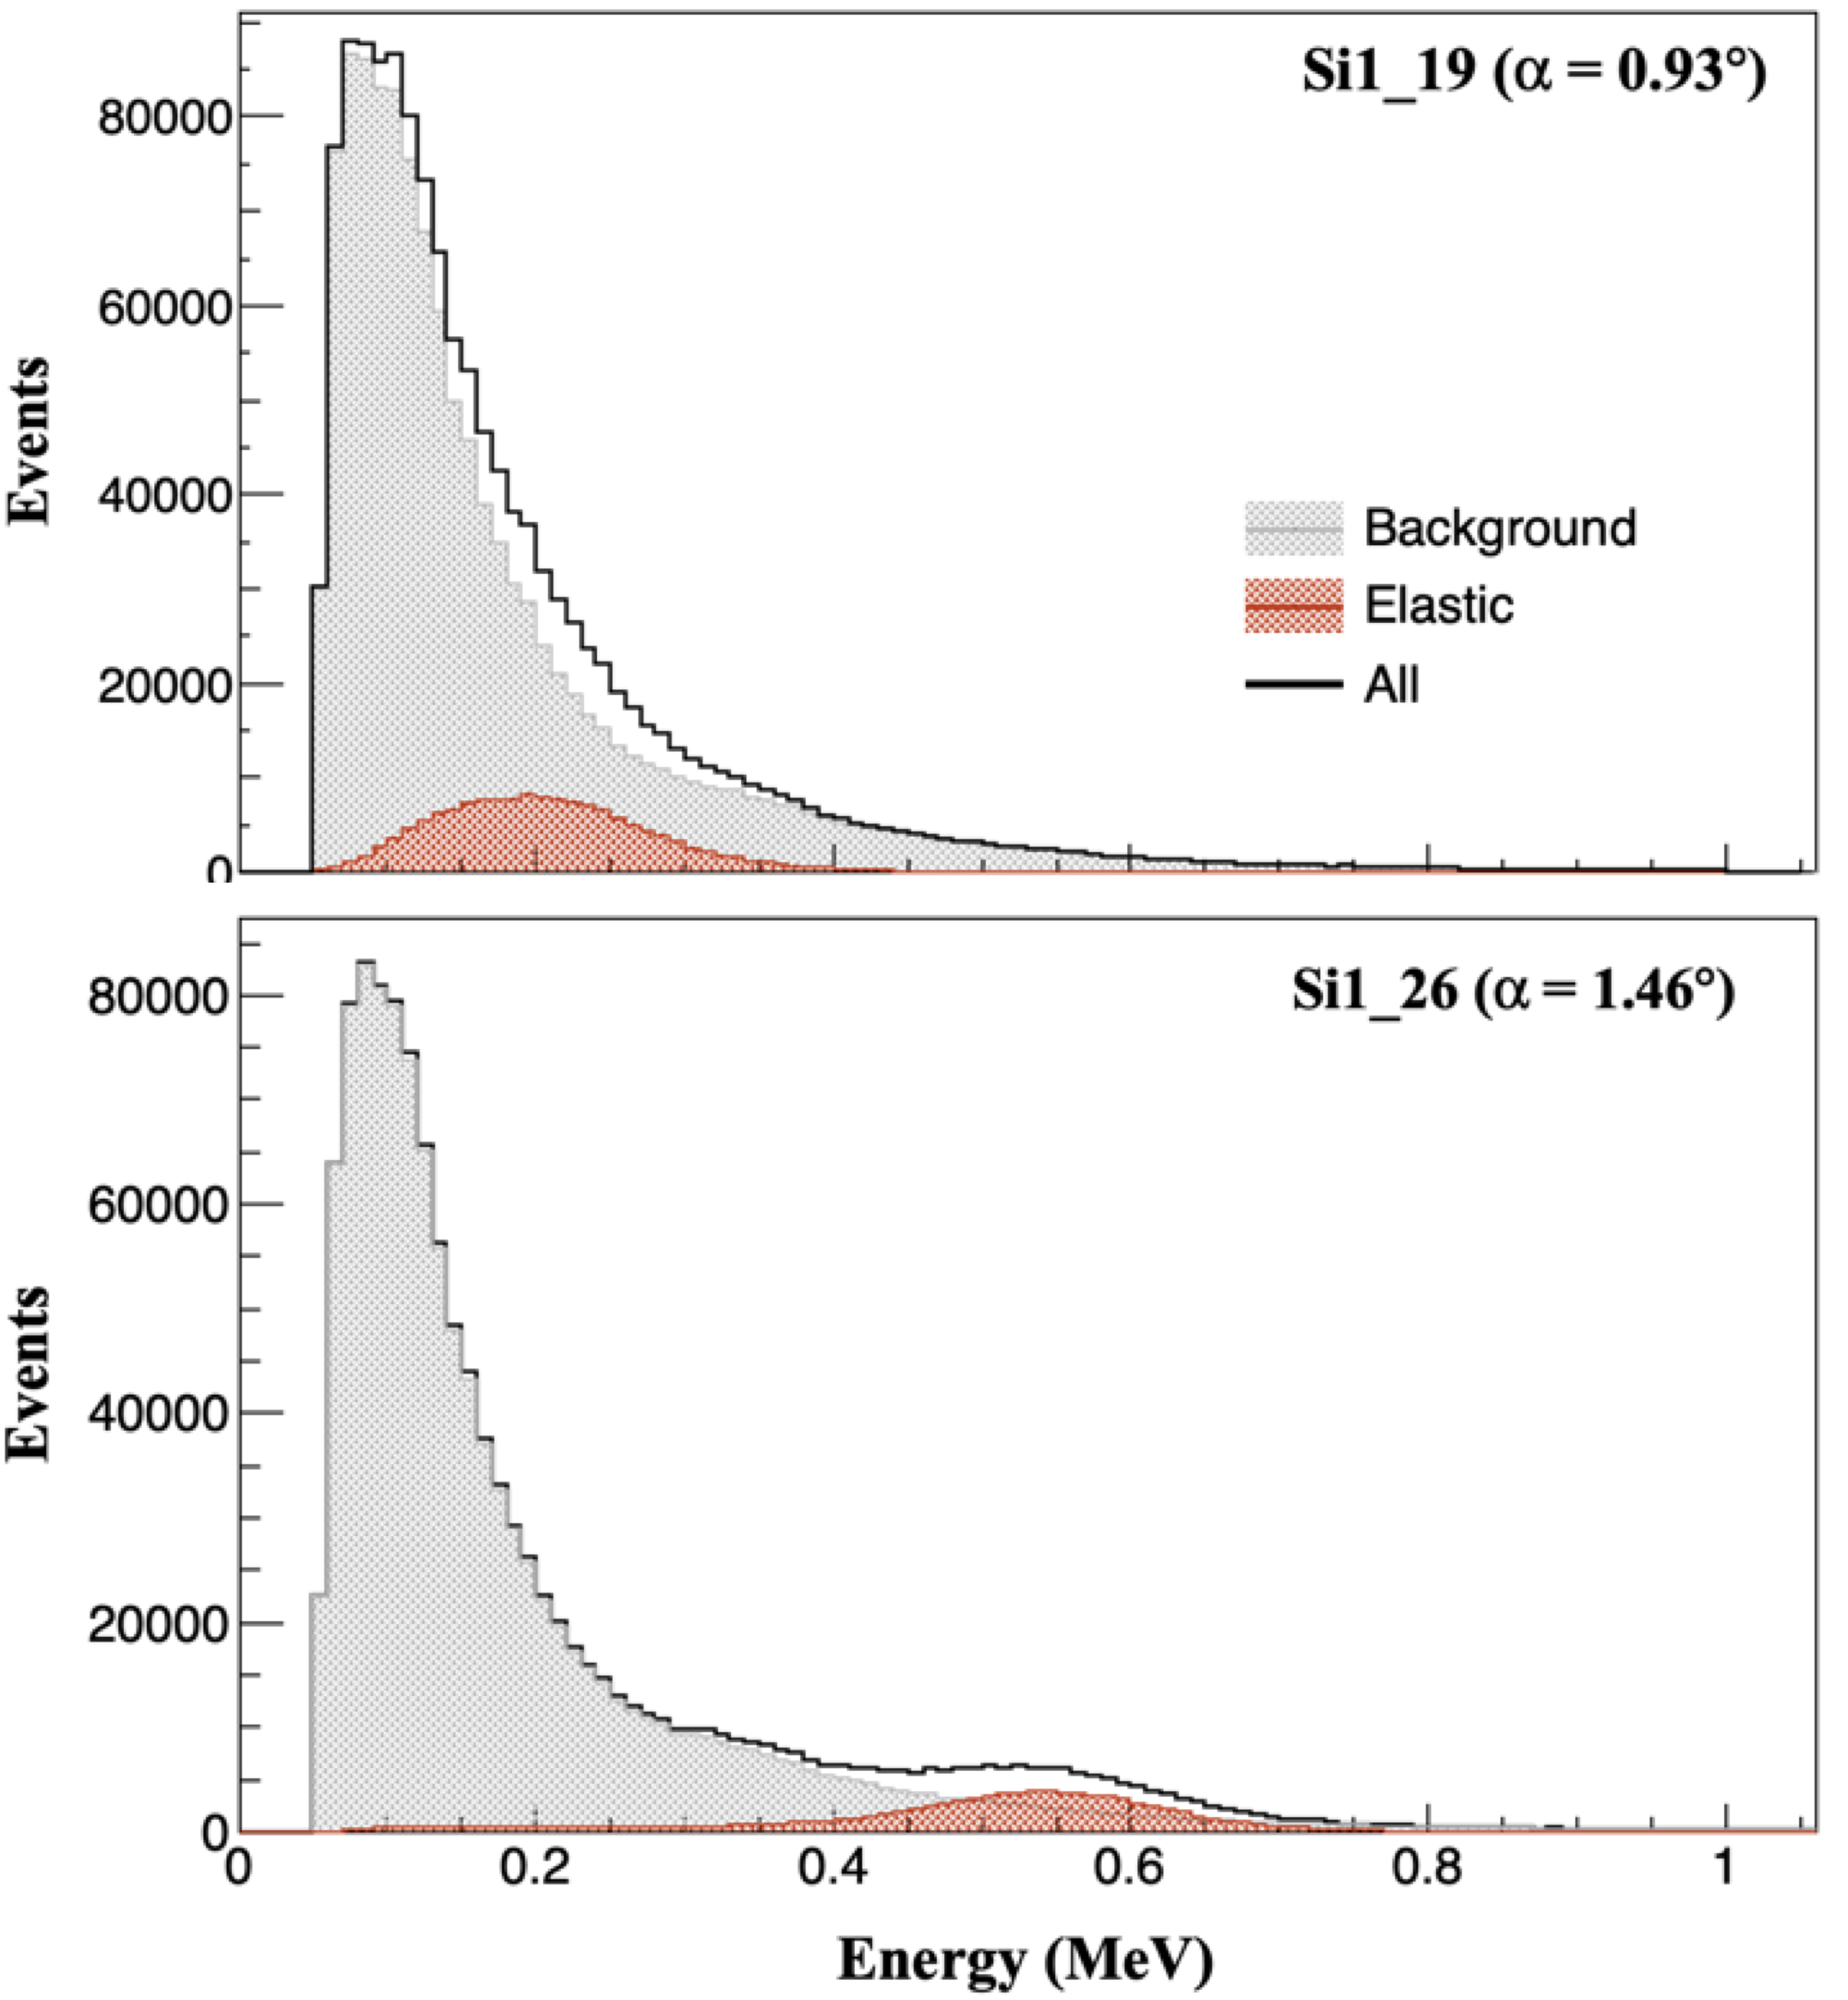
\includegraphics[width=0.45\textwidth]{./comparison_tof_e_cut_2.2_angle.png}
  \caption{Energy spectrums (black) of two channels at small recoil angle on Si1 (from
    $2.2 GeV/c$ data). The elastic peak (red) overlaps with the low-energy background
    spectrum (grey) and is hardly recognizable in the original spectrum. These low-energy background events are effectively surpressed by applying the TOF-E relation selection.}
  \label{fig:cut}
\end{figure}


\begin{figure}[h!]
  \centering
  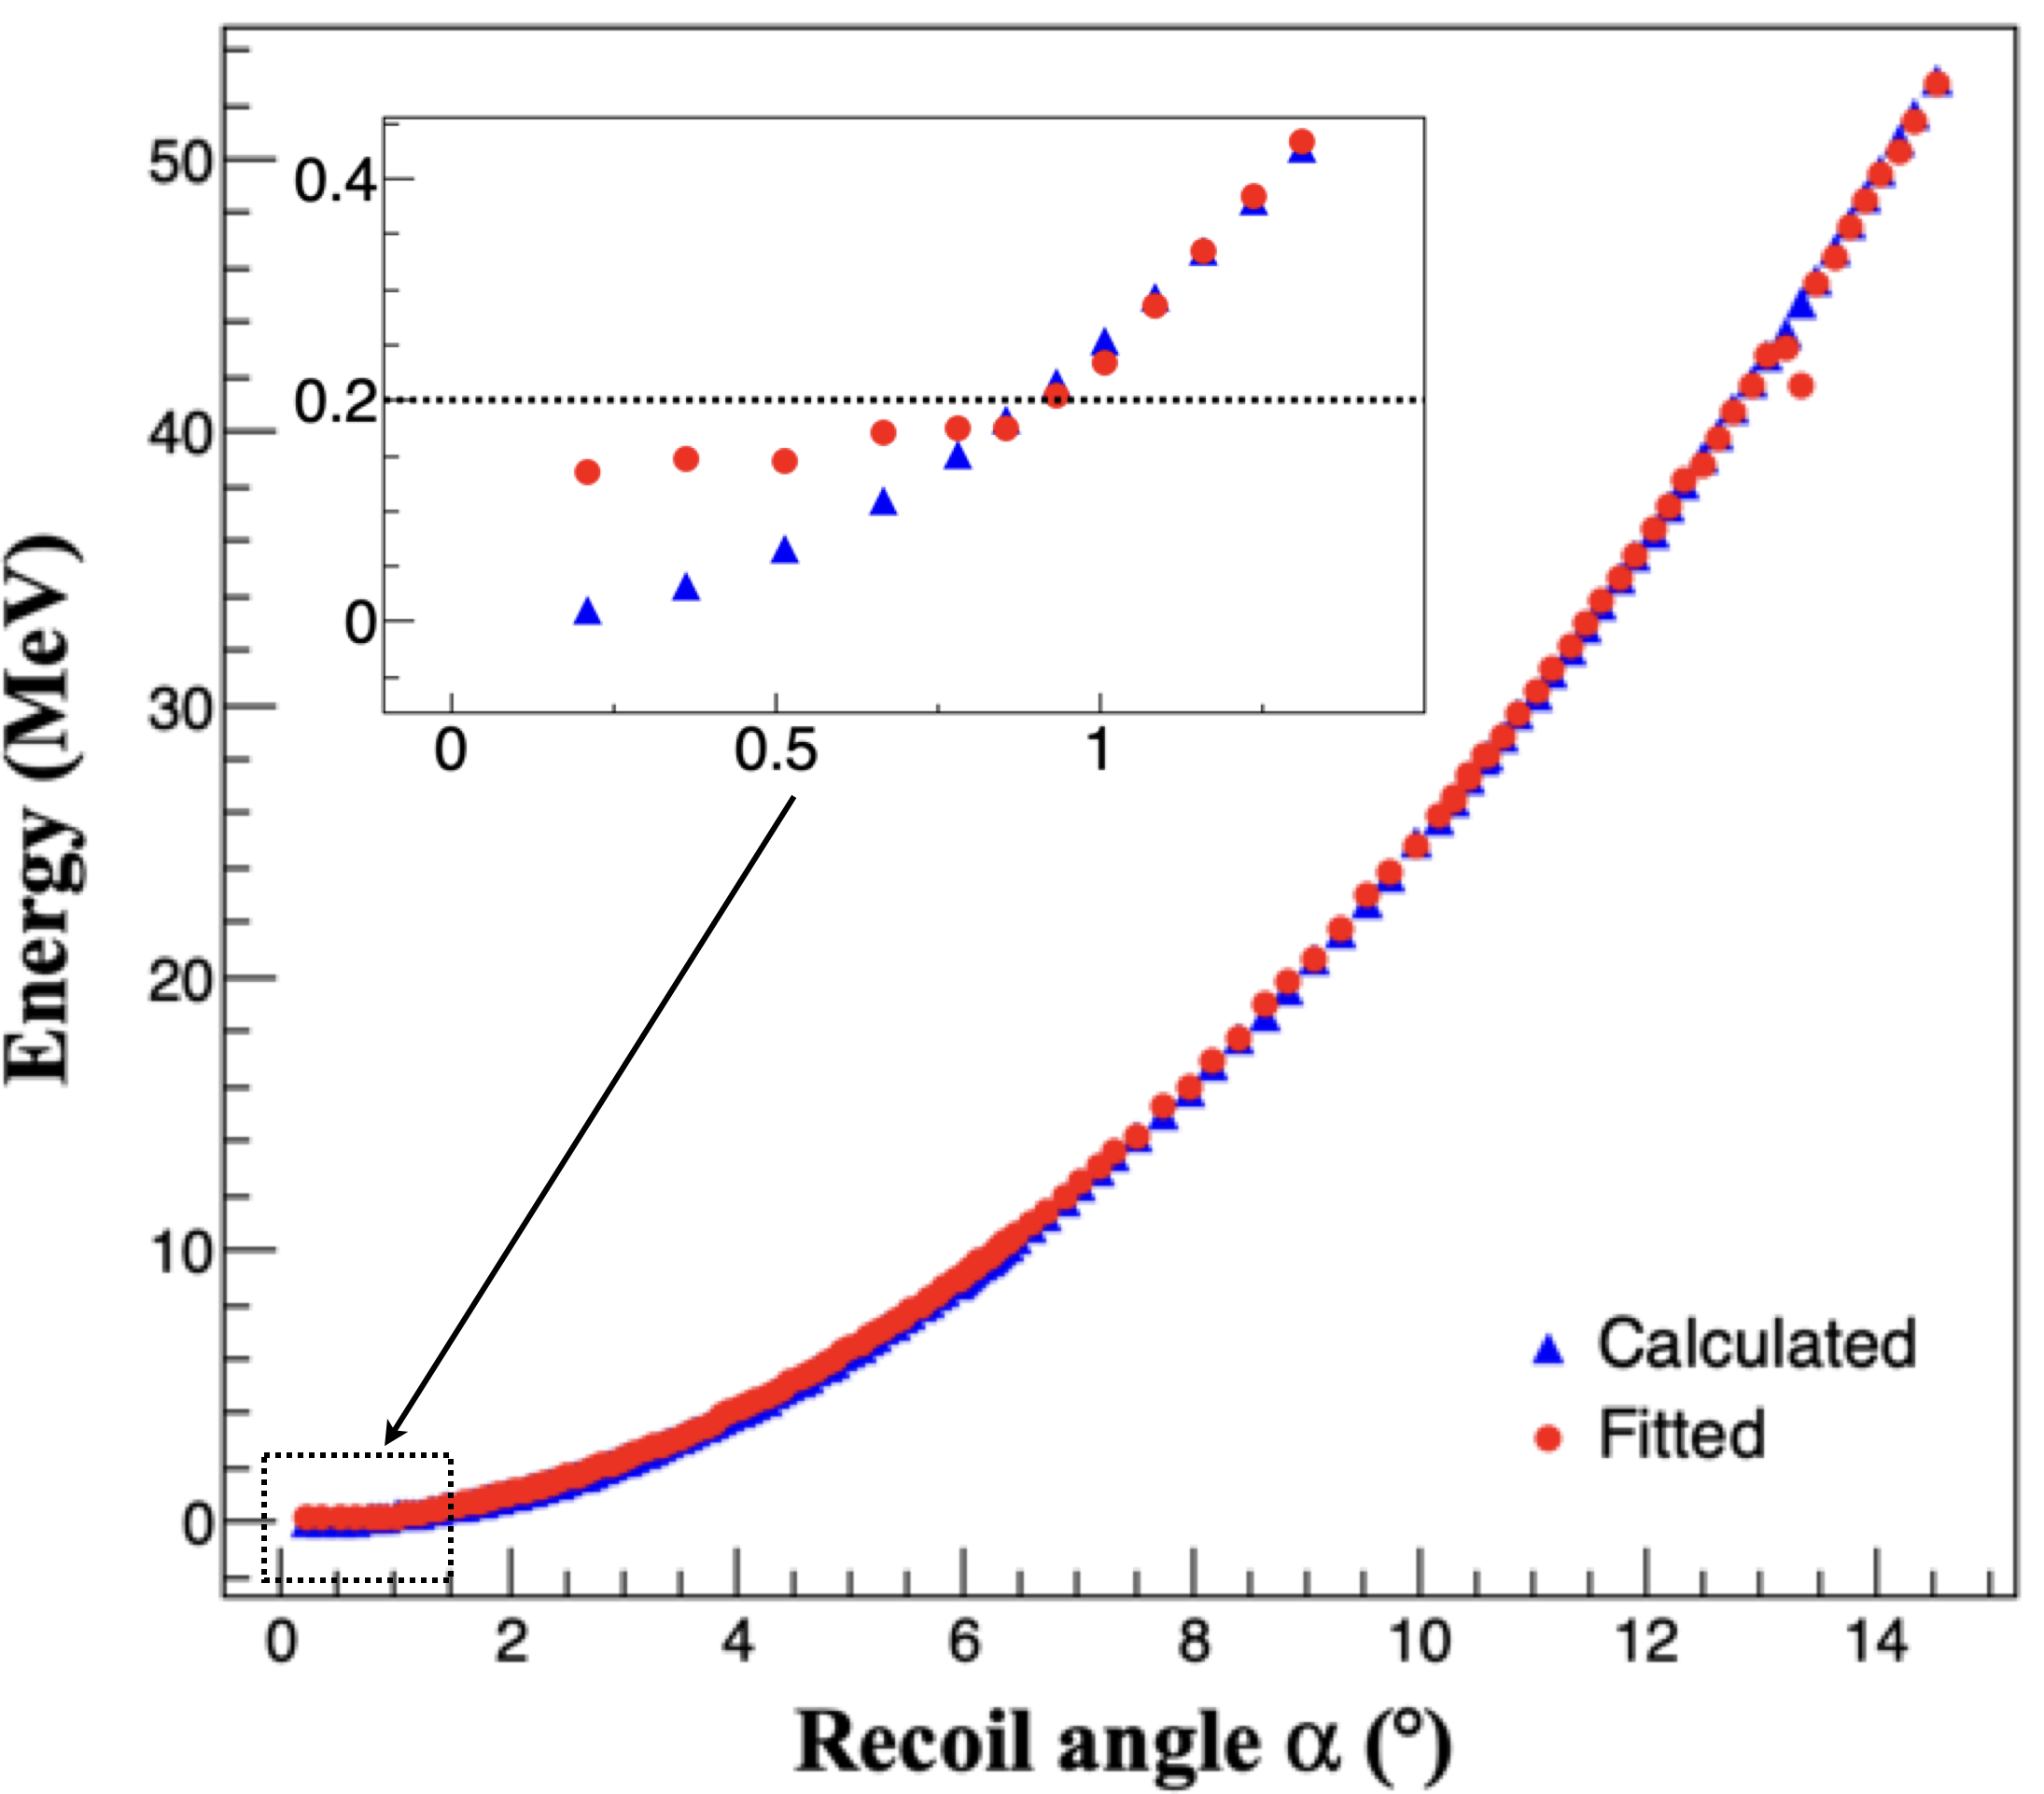
\includegraphics[width=0.42\textwidth]{./calc_vs_measured_2.2_angle_combined.png}
  \caption{
    Comparison of measured (red circle) and calculated (blue triangle) recoil energy with respect to the strip position along z-axis (i.e. beam direction) at beam momentum 2.2 GeV/c.}
  \label{fig:measured_vs_calculated}
\end{figure}


\section{Conclusion and Outlook}
\label{sec:conclusion}

The commissioning of the full KOALA setup at COSY, specifically of the new forward detector, is successful.
A strong correlation between the recoil detector and the forward detector is
observed for the covered region of the forward detector.
The idea of using the TOF-E relation of the recoil proton to extract elastic
scattering events is verified.
Preliminary analysis shows that lower |t| beyond the design requirement of 0.0008 (GeV/c)$^2$ can be reached from 2.2 to 3.0 GeV/c. 

However, it's also found that the forward detector could not cover the full
length of strips at larger recoil angles within the designed acceptance.
% that even in the forward-covered region, some elastic
% events do not generate coincidence between the recoil and forward detector.
This is mainly due to the fact that the stochastic cooling is not stable all the time
and the beam profile is larger than expected.
More strict requirement for the stochastic cooling is needed for future experiments.
Besides, scintillators with larger size, especially larger width, are also proposed.

The updated DAQ operated in stable condition in the commissioning tests.
But it's found that the limited performance of DAQ will bring an efficiency bias in different
sub-detectors due to the differenct noise triggering level.
Optimization of the DAQ is needed to minimize this bias.
The mask gate in the trigger logic is proposed to be removed in the future.
Thus, more tests of the timestamp-based synchronization in the offline analysis are needed.

\bibliographystyle{elsarticle-num}
\bibliography{reference}

\end{document}
